\documentclass[12pt,a4paper,twoside]{report}

% PACKAGE 
\usepackage{geometry}
\usepackage{setspace}
\usepackage{graphicx}
\usepackage{amsmath,amsfonts,amssymb}
\usepackage{url} 
\usepackage{hyperref} 
\usepackage{fancyhdr}
\usepackage{titlesec}
\usepackage{tocloft}
\usepackage{float}
\usepackage{array}
\usepackage{longtable}
\usepackage{afterpage}
\usepackage{etoolbox}
\usepackage{fontspec}   % XeLaTeX → tidak perlu inputenc/fontenc
\usepackage{tocbibind}
\usepackage{indentfirst}
\usepackage{caption}
\usepackage[indonesian]{babel}
\usepackage{enumitem}
\usepackage{tabularx}
\usepackage{ragged2e}
\usepackage[table]{xcolor}
\usepackage{multirow}
\usepackage{csquotes}
\usepackage{apalike}
\bibliographystyle{apalike}

% Set global style untuk enumerate & itemize
\setlist[enumerate]{leftmargin=1.25cm, topsep=0pt, itemsep=0pt, parsep=0pt, partopsep=0pt}
\setlist[itemize]{leftmargin=1.25cm, topsep=0pt, itemsep=0pt, parsep=0pt}

%  FORMAT LIST NAMES 
\addto\captionsindonesian{%
  \renewcommand{\contentsname}{DAFTAR ISI}%
  \renewcommand{\listfigurename}{DAFTAR GAMBAR}%
  \renewcommand{\listtablename}{DAFTAR TABEL}%
}

%caption
\captionsetup[figure]{name=Gambar,labelsep=period} % Gambar 1.1. Judul
\captionsetup[table]{name=Tabel,labelsep=period}   % Tabel 1.1. Judul

% Hilangkan chapter number default
\titleformat{\chapter}[display]
  {\centering\normalfont\bfseries\fontsize{14pt}{16pt}\selectfont}
  {BAB \Roman{chapter}} % --> nomor romawi, tanpa "1" lagi
  {0pt}
  {\vspace{0.5em}\MakeUppercase{}}
  [\vspace{1em}]

 

\titlespacing*{\chapter}{0pt}{-20pt}{20pt} % opsional atur jarak

% FORMAT CHAPTER (NO NUMBER) 
%\titleformat{name=\chapter,numberless}[display]
%  {\centering\normalfont\bfseries\fontsize{14pt}{16pt}\selectfont}
%  {}
%  {0pt}
%  {\vspace{0.5em}\MakeUppercase{#1}} % contoh: ABSTRAK, ABSTRACT
%  [\vspace{1em}]

% FORMAT SECTION 
\titleformat{\section}
  {\normalfont\bfseries\fontsize{13pt}{15pt}\selectfont}
  {\thesection}{1em}{}
\titlespacing*{\section}{0pt}{*1}{0pt} % hilangkan gap ke paragraf

% FORMAT SUBSECTION
\titleformat{\subsection}
  {\normalfont\bfseries\fontsize{12pt}{14pt}\selectfont}
  {\thesubsection}{1em}{}
\titlespacing*{\subsection}{0pt}{*1}{0pt} % hilangkan gap ke paragraf

% FORMAT PARAGRAF
\renewcommand\normalsize{\fontsize{12pt}{14pt}\selectfont} % isi 12 pt
\setlength{\parindent}{1.25cm} % masuk ke dalam
\setlength{\parskip}{0pt}


% SETUP 
\geometry{left=3cm,right=2cm,top=2.5cm,bottom=2.5cm}
\singlespacing
\setmainfont{Times New Roman}

% Hyperlink
\hypersetup{
    colorlinks=true,
    linkcolor=black,
    urlcolor=black,   % semua hitam
    citecolor=black,
    pdftitle={Proposal Tugas Akhir},
    pdfauthor={Nama Mahasiswa}
}

% Fancyhdr Styles
\fancypagestyle{romanstyle}{
  \fancyhf{}
  \fancyfoot[RO]{\thepage}
  \fancyfoot[LE]{\thepage}
  \renewcommand{\headrulewidth}{0pt}
  \renewcommand{\footrulewidth}{0pt}
}

\fancypagestyle{arabicstyle}{
  \fancyhf{}
  \fancyfoot[RO]{\thepage}
  \fancyfoot[LE]{\thepage}
  \renewcommand{\headrulewidth}{0pt}
  \renewcommand{\footrulewidth}{0pt}
}

\fancypagestyle{plain}{%
  \fancyhf{}%
  \fancyfoot[RO]{\thepage}%
  \fancyfoot[LE]{\thepage}%
  \renewcommand{\headrulewidth}{0pt}%
  \renewcommand{\footrulewidth}{0pt}%
}

% ==========================
% TOC, LOF, LOT Bahasa Indonesia
% ==========================
\renewcommand{\contentsname}{DAFTAR ISI}
\renewcommand{\listfigurename}{DAFTAR GAMBAR}
\renewcommand{\listtablename}{DAFTAR TABEL}

% Default: HILANGKAN titik-titik untuk entry chapter (dipakai utk yg sebelum Bab 1)
\renewcommand{\cftchapleader}{\hfill} % no dots
\renewcommand{\cftchappagefont}{\normalfont}
\renewcommand{\cftchapfont}{\normalfont\fontsize{11}{13}\normalcolor}

% Default chapter: tetap ada nomor di TOC
\renewcommand{\cftchappresnum}{BAB\ }
\renewcommand{\cftchapaftersnum}{}
\setlength{\cftchapnumwidth}{3em}

% Command entry TOC tanpa nomor
\newcommand{\tocnonum}[1]{%
  \addcontentsline{toc}{chapter}{#1}%
}


% Judul Daftar Isi, Gambar, Tabel (14pt, bold, tengah)
\renewcommand{\cfttoctitlefont}{\hfill\normalfont\fontsize{14}{17}\bfseries}
\renewcommand{\cftaftertoctitle}{\hfill}
\renewcommand{\cftloftitlefont}{\hfill\normalfont\fontsize{14}{17}\bfseries}
\renewcommand{\cftafterloftitle}{\hfill}
\renewcommand{\cftlottitlefont}{\hfill\normalfont\fontsize{14}{17}\bfseries}
\renewcommand{\cftafterlottitle}{\hfill}

% Isi Daftar Isi (11pt normal)
\renewcommand{\cftsecfont}{\normalfont\fontsize{11}{13}\normalcolor}
\renewcommand{\cftsubsecfont}{\normalfont\fontsize{11}{13}\normalcolor}
\renewcommand{\cftsubsubsecfont}{\normalfont\fontsize{11}{13}\normalcolor}
\renewcommand{\cftsecnumfont}{\normalfont\fontsize{11}{13}\normalcolor}
\renewcommand{\cftsubsecnumfont}{\normalfont\fontsize{11}{13}\normalcolor}
\renewcommand{\cftsubsubsecnumfont}{\normalfont\fontsize{11}{13}\normalcolor}

% Isi Daftar Gambar & Daftar Tabel (11pt normal, titik-titik aktif)
\renewcommand{\cftfigfont}{\normalfont\fontsize{11}{13}\normalcolor}
\renewcommand{\cftfignumfont}{\normalfont\fontsize{11}{13}\normalcolor}
\renewcommand{\cfttabfont}{\normalfont\fontsize{11}{13}\normalcolor}
\renewcommand{\cfttabnumfont}{\normalfont\fontsize{11}{13}\normalcolor}
\renewcommand{\cftfigleader}{\cftdotfill{\cftdotsep}}
\renewcommand{\cfttableader}{\cftdotfill{\cftdotsep}}

% mulai Bab I, pakai titik-titik 
\usepackage{etoolbox}
\pretocmd{\chapter}{%
  \renewcommand{\cftchapleader}{\cftdotfill{\cftdotsep}}%
}{}{}

%  VARIABEL 
\newcommand{\kodeTA}{EE234799}
\newcommand{\judulTA}{JUDUL PROPOSAL TUGAS AKHIR DITULIS DALAM \\ KAPITAL DAN KATA ASING DITULIS DALAM \textit{ITALIC}}
\newcommand{\namaMhs}{NAMA MAHASISWA}
\newcommand{\nrpMhs}{5022XXXXXX}
\newcommand{\pembimbingSatu}{Nama Pembimbing Satu dan Gelar}
\newcommand{\nipPembimbingSatu}{XXXXXXXXXXXXXXXXXX}
\newcommand{\pembimbingDua}{Nama Pembimbing Dua dan Gelar}
\newcommand{\nipPembimbingDua}{XXXXXXXXXXXXXXXXXX}
\newcommand{\prodi}{Program Studi Sarjana (S1) Teknik Elektro}
\newcommand{\depart}{Departemen Teknik Elektro}
\newcommand{\fakul}{Fakultas Teknologi Elektro dan Informatika Cerdas}
\newcommand{\kampus}{Institut Teknologi Sepuluh Nopember}
\newcommand{\kota}{Surabaya}
\newcommand{\tahundibuat}{20XX}
\newcommand{\judulinggris}{THE TITLE OF THE FINAL PROJECT PROPOSAL IS WRITTEN IN CAPITAL LETTERS AND ENGLISH WORDS DO NOT NEED ITALIC}
\newcommand{\namamhs}{Nama Mahasiswa}
\newcommand{\pengujisatu}{Nama dan gelar penguji satu}
\newcommand{\pengujidua}{Nama dan gelar penguji dua}
\newcommand{\pengujitiga}{Nama dan gelar penguji tiga}
\newcommand{\bulandibuat}{Bulan}
\newcommand{\titikTiga}{\textellipsis}

% DOKUMEN
\begin{document}

% Cover (tidak masuk daftar isi)
% COVER PAGE
\begin{titlepage}

% khusus cover font yg digunakan adalah Trebuchet MS (bagian lain menggunakan Times New Roman)
\fontspec{Trebuchet MS}

% Logo pojok kiri atas
\vspace*{-1.5cm} % geser naik 
\noindent

\includegraphics[width=2.5cm]{cover/logoITS.png} \\[1cm] 

% Garis biru 
\definecolor{ITSBlue}{RGB}{0,114,198}
\noindent\hspace*{-3cm}\textcolor{ITSBlue}{\rule{\paperwidth}{1cm}} \\[0.3cm]

% Kode TA
\noindent
{\fontsize{14pt}{14pt}\selectfont \textbf{PROPOSAL TUGAS AKHIR – \kodeTA}} \\[2cm]

% Judul
\noindent
{\fontsize{18pt}{14pt}\selectfont \textbf{\judulTA}} \\[2cm]

% Nama mahasiswa
\noindent
{\fontsize{14pt}{14pt}\selectfont \textbf{\namaMhs} \\ NRP \nrpMhs} \\[2cm]

% Dosen pembimbing
\noindent
{\fontsize{14pt}{14pt}\selectfont Dosen Pembimbing} \\[0.3cm]
\noindent
{\fontsize{14pt}{14pt}\selectfont \textbf{\pembimbingSatu} \\ NIP \nipPembimbingSatu} \\[0.8cm]
\noindent
{\fontsize{14pt}{14pt}\selectfont \textbf{\pembimbingDua} \\ NIP \nipPembimbingDua} \\[2cm]

% Program studi
\noindent
{\fontsize{12pt}{14pt}\selectfont \textbf{\prodi}} \\[0.3cm]
\noindent
{\fontsize{12pt}{14pt}\selectfont
\depart \\
\fakul \\
\kampus \\
\kota \\
\tahundibuat}

% Kembalikan font default (Times New Roman) setelah cover
\normalfont

\end{titlepage}

\clearpage
\thispagestyle{empty}
\vspace*{\fill}
\begin{center}
    {\fontsize{12pt}{14pt}\selectfont \textit{Halaman ini sengaja dikosongkan}}
\end{center}
\vspace*{\fill}
\clearpage


\pagestyle{romanstyle}
\pagenumbering{roman}

\addcontentsline{toc}{chapter}{LEMBAR PENGESAHAN}
\clearpage
\thispagestyle{romanstyle} % biar nomor muncul sesuai aturan fancyhdr

\begin{center}

% Judul
{\fontsize{14pt}{14pt}\selectfont \textbf{LEMBAR PENGESAHAN}} \\[1.5cm]

% Judul proposal
{\fontsize{12pt}{14pt}\selectfont \textbf{\judul}} \\[1.5cm]

% Keterangan proposal
{\fontsize{12pt}{14pt}\selectfont \textbf{PROPOSAL TUGAS AKHIR} \\
Diajukan untuk memenuhi salah satu syarat \\
memperoleh gelar Sarjana Teknik pada \\
Program Studi Sarjana \\
\depart \\
\fakul \\
\kampus } \\[1cm]

% Nama mahasiswa
{\fontsize{12pt}{14pt}\selectfont Oleh: \textbf{\namaMhs}} \\
{\fontsize{12pt}{14pt}\selectfont NRP. \nrpMhs } \\[1cm]

% Persetujuan penguji
{\fontsize{12pt}{14pt}\selectfont Disetujui oleh Tim Penguji Proposal Tugas Akhir:} \\[1.5cm]

% Tabular dengan titik rapi
\begin{tabular}{p{0.5cm} p{7cm} p{3.5cm} p{3cm}}
1. & \pembimbingSatu & Pembimbing & \titikTiga \\[1.5cm]
2. & \pembimbingDua  & Ko-Pembimbing & \titikTiga \\[1.5cm]
3. & \pengujisatu    & Penguji & \titikTiga \\[1.5cm]
4. & \pengujidua     & Penguji & \titikTiga \\[1.5cm]
5. & \pengujitiga    & Penguji & \titikTiga \\[1.5cm]
\end{tabular}

\vfill

% Kota, bulan, tahun
{\fontsize{12pt}{14pt}\selectfont \textbf{SURABAYA}} \\
{\fontsize{12pt}{14pt}\selectfont \bulandibuat, \tahundibuat}

\end{center}

\clearpage


\newpage
\clearpage
\thispagestyle{romanstyle} % ada nomor romawi
\vspace*{\fill}
\begin{center}
    {\fontsize{12pt}{14pt}\selectfont \textit{Halaman ini sengaja dikosongkan}}
\end{center}
\vspace*{\fill}
\clearpage


\addcontentsline{toc}{chapter}{ABSTRAK}
\clearpage
\thispagestyle{romanstyle} % nomor halaman romawi

\begin{center}
{\bfseries \judulTA} \\[1cm]
\end{center}

\noindent
\begin{tabular}{l l l}
\textbf{Nama Mahasiswa/NRP} & \textbf{:} & \textbf{\namamhs}/\textbf{\nrpMhs} \\
\textbf{Departemen}         & \textbf{:} & \textbf{\depart} \\
\textbf{Dosen Pembimbing}   & \textbf{:} & \textbf{\pembimbingSatu} \\
                            &            & \textbf{\pembimbingDua}
\end{tabular}


\vspace{1cm}

\vspace{1cm}

\noindent {\bfseries Abstrak} % judul ABSTRAK rata kiri, tanpa inden
\par % akhiri baris judul suapaya bawahnya ga ikutan

\setlength{\parindent}{1.25cm} % panjang inden paragraf
Abstrak ditulis dalam satu paragraf tunggal, berisi tentang hal-hal yang akan dikerjakan pada pelaksanaan Tugas Akhir yang terdiri dari 200-300 kata. Abstrak merupakan ringkasan rencana penelitian/rencana rancangan/proyek, yang berisi jawaban atas pertanyaan, apa, mengapa, dan bagaimana penelitian/rancangan yang akan dilakukan. Dalam sebuah abstrak, biasanya dijelaskan secara singkat latar belakang masalah yang diteliti, tujuan penelitian, metode yang digunakan, hasil utama yang diperoleh, serta kesimpulan yang diambil dari hasil penelitian tersebut. Abstrak yang baik harus ditulis dengan jelas dan padat, mencerminkan seluruh isi karya tulis secara akurat, serta mampu menarik minat pembaca untuk mendalami lebih lanjut penelitian yang dilakukan. Sebagai elemen penting dari karya ilmiah, abstrak sering kali menjadi bagian yang pertama kali dilihat oleh pembaca, sehingga kualitas penulisannya sangat krusial. Penulisan kata kunci dimulai dari abjad yang paling awal dan apabila terdapat kata dalam bahasa asing harap dimiringkan.

\vspace{0.5cm}
\noindent
{\bfseries Kata kunci:} Abstrak, Menarik, Padat, Penting, Singkat
 
\newpage
\clearpage
\thispagestyle{romanstyle} % ada nomor romawi
\vspace*{\fill}
\begin{center}
    {\fontsize{12pt}{14pt}\selectfont \textit{Halaman ini sengaja dikosongkan}}
\end{center}
\vspace*{\fill}
\clearpage


\addcontentsline{toc}{chapter}{ABSTRACT}
\clearpage
\thispagestyle{romanstyle} % nomor halaman romawi

\begin{center}
{\bfseries \judulinggris} \\[1cm]
\end{center}

\noindent
\begin{tabular}{l l l}
\textbf{Student Name/NRP} & \textbf{:} & \textbf{\namamhs}/\textbf{\nrpMhs} \\
\textbf{Department}         & \textbf{:} & \textbf{\depart} \\
\textbf{Advisor}   & \textbf{:} & \textbf{\pembimbingSatu} \\
                   &            & \textbf{\pembimbingDua}
\end{tabular}


\vspace{1cm}

\noindent {\bfseries Abstrak} % judul ABSTRAK rata kiri, tanpa inden
\par % akhiri baris judul suapaya bawahnya ga ikutan
\setlength{\parindent}{1.25cm} % panjang inden paragraf
The abstract is written in a single paragraph, containing information about the work to be carried out in the Final Project, consisting of 200-300 words. The abstract is a summary of the research plan/design plan/project, which contains answers to the questions of what, why, and how the research/design will be carried out. In an abstract, the background of the problem being studied, the research objectives, the methods used, the main results obtained, and the conclusions drawn from the research results are usually explained briefly. A good abstract should be written clearly and concisely, accurately reflecting the entire content of the paper, and be able to attract readers' interest to explore the research further. As an important element of scientific work, the abstract is often the first part that readers see, so the quality of its writing is crucial. Keywords should be written in alphabetical order, and if there are words in a foreign language, they should be italicised.


\vspace{0.5cm}
\noindent
{\bfseries Keywords: Abstract, Interesting, Concise, Important, Brief} 
 
\newpage
\clearpage
\thispagestyle{romanstyle} % ada nomor romawi
\vspace*{\fill}
\begin{center}
    {\fontsize{12pt}{14pt}\selectfont \textit{Halaman ini sengaja dikosongkan}}
\end{center}
\vspace*{\fill}
\clearpage


% Daftar isi, gambar, tabel (otomatis masuk ke ToC)
\tableofcontents
\newpage
\clearpage
\thispagestyle{romanstyle} % ada nomor romawi
\vspace*{\fill}
\begin{center}
    {\fontsize{12pt}{14pt}\selectfont \textit{Halaman ini sengaja dikosongkan}}
\end{center}
\vspace*{\fill}
\clearpage


\listoffigures
\newpage
\clearpage
\thispagestyle{romanstyle} % ada nomor romawi
\vspace*{\fill}
\begin{center}
    {\fontsize{12pt}{14pt}\selectfont \textit{Halaman ini sengaja dikosongkan}}
\end{center}
\vspace*{\fill}
\clearpage


\listoftables
\newpage
\clearpage
\thispagestyle{romanstyle} % ada nomor romawi
\vspace*{\fill}
\begin{center}
    {\fontsize{12pt}{14pt}\selectfont \textit{Halaman ini sengaja dikosongkan}}
\end{center}
\vspace*{\fill}
\clearpage


% ISI
\clearpage
\pagestyle{arabicstyle}
\pagenumbering{arabic}

\chapter{PENDAHULUAN}

\section{Latar Belakang}
Bagian ini secara umum berisi latar belakang dan alasan penulis memilih objek penelitian. Uraian dimulai dengan penjelasan mengenai hal yang bersifat umum terkait dengan topik Tugas Akhir (TA), kemudian diarahkan kepada hal yang lebih khusus yaitu judul proposal TA. Objek yang akan diteliti harus dijelaskan secara konkret sebagai pengantar menuju permasalahan, dan sebagai hasil kajian/studi terdahulu/hasil analisis atas data sekunder, tentang obyek yang akan diteliti/dirancang, disertai alasan mengapa masalah tersebut perlu diteliti baik secara teoritis maupun praktis. 
%pergantian paragraf
Latar belakang tugas akhir biasanya berisi gap analysis yang fungsinya untuk mengidentifikasi dan menjelaskan kesenjangan antara kondisi atau pengetahuan yang ada dengan kondisi ideal atau yang diinginkan. Dalam konteks penelitian, gap analysis membantu mengungkapkan area di mana penelitian sebelumnya belum memadai, atau ada aspek yang belum terjelaskan dengan baik. Dengan demikian, latar belakang tugas akhir menjelaskan mengapa penelitian ini penting dilakukan untuk mengisi kesenjangan tersebut, sekaligus membuktikan relevansi dan kontribusi dari penelitian yang diusulkan. Hal ini memperkuat argumen tentang nilai dan urgensi penelitian yang akan dilakukan. Tambahkan gambar apabila diperlukan. Contoh tampilan gambar dapat dilihat pada Gambar \ref{fig:kapasitor}.


\begin{figure}[h!]
    \centering
    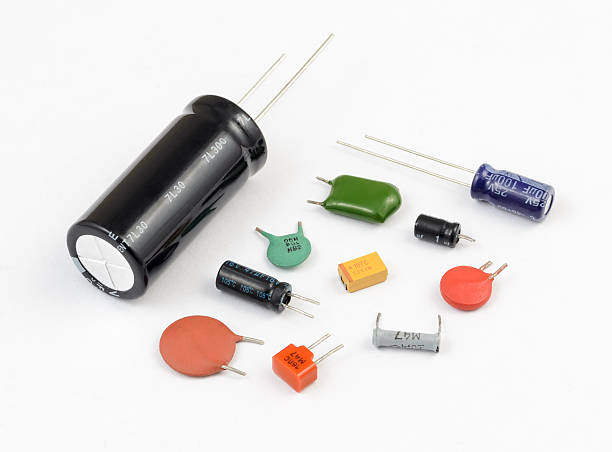
\includegraphics[width=0.7\textwidth]{gambar/kapasitor.jpg}
    \caption{Jenis Kapasitor di Dunia Elektro}
    \label{fig:kapasitor}
\end{figure}

\section{Rumusan Masalah}
Permasalahan penelitian harus dituliskan dalam bentuk deklaratif atau kalimat-kalimat pertanyaan yang tegas dan jelas. Masalah penelitian merupakan perumusan kesenjangan antara keadaan yang ada dengan keadaan yang ingin dicapai. Perumusan masalah dilakukan berdasarkan identifikasi masalah dan ruang lingkup penelitian yang akan dipecahkan. Perumusan masalah ini dituangkan dalam bentuk pertanyaan yang nantinya akan dijawab di dalam analisis masalah dengan menggunakan teori atau konsep yang relevan dan didukung oleh data pada pelaksanaan penelitian yang akan dilakukan. Dalam merumuskan masalah perlu dihindari mengemukakan banyak pertanyaan, yang artinya bahwa rumusan masalah tidak dituliskan dalam bentuk pertanyaan yang terlalu banyak jumlahnya.

\section{Batasan Masalah}
Ruang lingkup/pembatasan masalah dalam upaya memfokuskan penelitian yang akan dilakukan menjadi lebih terarah. Pembatasan dapat dilakukan dari segi keluasan, kedalaman, kemampuan peneliti dalam aspek tertentu, atau semua segi tersebut. Pembatasan harus disertai alasan atau argumentasi mengapa pembatasan masalah perlu dilakukan. Batasan masalah terkait dengan variable penelitian/variabel perancangan, variabel dan/atau parameter terhadap variabel penelitian/perancangan, dan/atau variabel/parameter yang diasumsikan sebagai parameter konstanta atau parameter yang diabaikan.

\section{Tujuan}
Tujuan penelitian/perancangan berisi uraian tentang tujuan penulis melakukan penelitian/perancangan, yaitu untuk menjawab pertanyaan yang telah dituliskan di dalam bagian perumusan masalah atau hasil yang akan dicapai atau jawaban permasalahan penelitian/perancangan. Tujuan penelitian/perancangan dapat dituliskan dalam serangkaian tujuan, yang merupakan tujuan yang lebih spesifik, yang mendukung tujuan penelitian/perancangan. Pada bagian tujuan ini biasanya dapat dituliskan dalam bentuk poin-poin seperti contoh berikut:
\begin{enumerate}[leftmargin=1.25cm] % sejajar dengan paragraf/sub-bab
    \item Untuk mengembangkan...;
    \item Untuk mengidentifikasi...;
    \item Untuk mengukur...;
    \item Untuk menentukan...;
    \item Untuk membandingkan.... 
\end{enumerate}
\section{Manfaat}
Pada bagian ini diuraikan secara singkat tetapi jelas kontribusi hasil penelitian/perancangan terhadap pengembangan bidang ilmu, teknologi, seni dan atau terhadap pemecahan persoalan pembangunan, dan atau terhadap pengembangan institusi.

\chapter{TINJAUAN PUSTAKA}

\section{Hasil Studi Terdahulu}
Hasil studi terdahulu merupakan penelitian/perancangan yang relevan yang pernah dilakukan oleh berbagai pihak, dan apabila memungkinkan bukan hasil pelaksanaan Tugas Akhir (TA) terdahulu, melainkan dari jurnal ilmiah, paten, atau laporan perancangan lainnya dari lembaga yang kredibel. Hasil studi terdahulu ditulis dalam bentuk parafrasae bukan menjiplak karya dari orang lain yang bisa dibuat dalam bentuk tabel seperti Tabel 2.1, atau dalam bentuk uraian (bukan tabel).
\captionsetup[table]{position=top,justification=centering}
\begin{table}[ht]
\caption{Hasil Studi Terdahulu}
\centering
\renewcommand{\arraystretch}{1.3} % biar tinggi baris agak lega
% Definisi kolom untuk justified text
\newcolumntype{Z}{>{\justifying\arraybackslash}X}
\begin{tabularx}{\textwidth}{|c|l|Z|}
\hline
\textbf{No} & \textbf{Penulis, tahun} & \textbf{Hasil Penelitian} \\ \hline
1 & Ghalindri, 2022 & 
Analisis perbandingan waktu dan biaya dilaksanakan pada pekerjaan pondasi yang membandingkan penggunaan spun pile dan bore pile pada Proyek Bangunan Penunjang Skybridge Proyek Stasiun Integrasi LRT Halim, Jakarta. Berdasarkan hasil penelitian didapatkan kebutuhan waktu pemancangan dengan menggunakan spun pile 19 hari lebih cepat daripada bore pile. Sedangkan dari aspek biaya diperoleh penghematan sebesar 60,96\% dari Rencana Anggaran Biaya (RAB) awal sebesar Rp. 3.259.073.514,00 menjadi Rp. 1.986.593.514,00. \\ \hline
2 & Annisa, 2022 & 
Analisis perbandingan waktu dan biaya dilaksanakan pada pekerjaan bekisting yang membandingkan penggunaan bekisting konvensional dan aluminium formwork pada proyek Trans Icon Surabaya. Dari hasil penelitian didapatkan selisih pekerjaan menggunakan kedua metode dari segi biaya sebesar Rp. 600.732.246,00 lebih murah dan dari segi waktu 73 hari lebih cepat dengan menggunakan bekisting aluminium formwork. \\ \hline
\end{tabularx}
\end{table}

\section{Perencanaan Struktur Sekunder (Contoh)}
\subsection{Perencanaan Tangga Baja (Contoh)}
Berdasarkan SNI 1729:2015, penampang yang mengalami tekuk lokal dikategorikan sebagai 
elemen nonlangsing penampang elemen langsing. Untuk profil elemen nonlangsing, rasio 
tebal-terhadap-lebar dari elemen tekan tidak boleh melebihi batas elastisitas kelangsingan 
untuk elemen non kompak $\lambda_r$. Apabila rasio tersebut melebihi $\lambda_r$, disebut 
penampang dengan elemen langsing. Parameter batas kelangsingan elemen nonkompak 
$\lambda_r$ dapat dihitung dengan persamaan \eqref{eq:rumus}.
\begin{equation}
    \lambda_r = 1.49 \sqrt{\frac{E}{F_y}}
    \label{eq:rumus}
\end{equation}
\noindent
Keterangan:
\begin{itemize}[label={},leftmargin=\parindent,itemsep=2pt,topsep=2pt]
  \item $\lambda_r$ = Parameter batas kelangsingan untuk elemen nonkompak
  \item $E$ = Modulus elastisitas baja = 200000 MPa
  \item $F_y$ = Tegangan leleh minimum yang disyaratkan (MPa)
\end{itemize}

\subsection{Perencanaan Plat Lantai (Contoh)}
Berdasarkan SNI 1729:2015, penampang Syang mengalami tekuk lokal dikategorikan sebagai elemen nonlangsing penampang elemen-langsing. Untuk profil elemen nonlangsing, rasio tebal-terhadap-lebar dari elemen tekan tidak boleh melebihi batas elastisitas kelangsingan untuk elemen non kompak λr. Apabila rasio tersebut melebihi λr, disebut penampang dengan elemen-langsing. Menurut \cite{alexandersadiku}, kapasitor terdiri dari dua plat konduktor. Sedangkan menurut \cite{varaprasad}, kapasitor mampu menyimpan muatan listrik.



\chapter{METODOLOGI}

\section{Tahap Pelaksanaan Studi}
Metodologi berisi penjelasan untuk mengartikulasikan rencana penelitan/perancangan dengan cukup jelas dan detil. Metodologi penelitian/perancangan/pembangunan alat memiliki banyak dimensi dan metode penelitian/perancangan/pembangunan alat merupakan bagian dari metodologi penelitian/perancangan/pembangunan alat. Salah satu contoh metodologi penelitian dapat dilihat pada Gambar \ref{fig:diagram}.

\begin{figure}[h!]
    \centering
    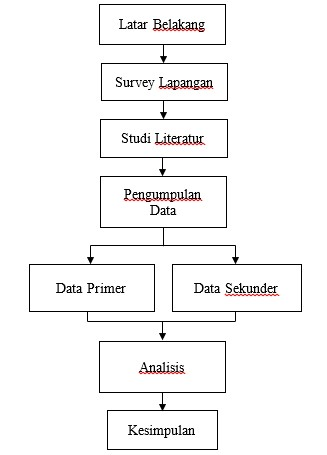
\includegraphics[width=0.6\textwidth]{gambar/diagram.jpg}
    \caption{Diagram Alir Penelitian}
    \label{fig:diagram}
\end{figure}

\section{Data Penelitian}
Data penelitian adalah informasi yang dikumpulkan, diukur, dan dianalisis selama proses penelitian. Data ini digunakan untuk menjawab pertanyaan penelitian, menguji hipotesis, atau membangun teori. Data penelitian yang digunakan berupa data primer maupun data sekunder Contoh data penelitian sekunder dapat dilihat pada Lampiran 1.

\section{...} % disesuaikan dengan metodologi yang digunakan

\section{...} % disesuaikan dengan metodologi yang digunakan

\section{Jadwal Pelaksanaan TA}
\definecolor{ITSBlue}{RGB}{0,114,198}
\renewcommand{\arraystretch}{1.3} % spasi antar baris
\setlength{\tabcolsep}{4pt}       % spasi antar kolom

\begin{tabularx}{\textwidth}{|p{4cm}|*{6}{>{\centering\arraybackslash}X|}}
\hline
\textbf{Kegiatan} & \multicolumn{6}{c|}{\textbf{Bulan}} \\ 
\cline{2-7}
 & 1 & 2 & 3 & 4 & 5 & 6 \\ \hline
Studi Literatur     & \cellcolor{ITSBlue} & \cellcolor{ITSBlue} &   &   &   &   \\ \hline
Perancangan Alat    &   & \cellcolor{ITSBlue} & \cellcolor{ITSBlue} &   &   &   \\ \hline
Pengujian           &   &   &   & \cellcolor{ITSBlue} & \cellcolor{ITSBlue} &   \\ \hline
Analisis Data       &   &   &   &   & \cellcolor{ITSBlue} & \cellcolor{ITSBlue} \\ \hline
Penyusunan Laporan  &   &   &   &   &   & \cellcolor{ITSBlue} \\ \hline
\end{tabularx}

\clearpage
\addcontentsline{toc}{chapter}{DAFTAR PUSTAKA}
\renewcommand{\bibname}{DAFTAR PUSTAKA}
\bibliography{pustaka}
\clearpage
\thispagestyle{arabicstyle} % ada nomor arabic
\vspace*{\fill}
\begin{center}
    {\fontsize{12pt}{14pt}\selectfont \textit{Halaman ini sengaja dikosongkan}}
\end{center}
\vspace*{\fill}
\clearpage
 %dikasih halaman kosong setiap bab yg berakhir pada halaman ganjil

% panggil file lampiran
\addcontentsline{toc}{chapter}{LAMPIRAN 1}
\clearpage
\appendix % masuk mode lampiran
\renewcommand{\thechapter}{\arabic{chapter}} % pastikan pakai angka

\begin{center}
% Judul
{\fontsize{14pt}{14pt}\selectfont \textbf{LAMPIRAN 1}} \\[1.5cm]
\end{center}


%\chapter*{Lampiran 1} % tidak ikut counter bab
%\addcontentsline{toc}{chapter}{Lampiran 1} % masuk daftar isi manual

\renewcommand{\arraystretch}{1.2}

\noindent
\begin{tabularx}{\textwidth}{|c|>{\centering\arraybackslash}X|
                                    >{\centering\arraybackslash}X|
                                    >{\centering\arraybackslash}X|
                                    >{\centering\arraybackslash}X|
                                    >{\centering\arraybackslash}X|}
\hline
No. & Segmen & As & Panjang & Jumlah & Volume \\
\hline
1 & & & & & \\
\hline
2 & & & & & \\
\hline
3 & & & & & \\
\hline
\end{tabularx}
 
\newpage

\end{document}
